\let\negmedspace\undefined
\let\negthickspace\undefined
\documentclass[journal]{IEEEtran}
\usepackage[a5paper, margin=10mm, onecolumn]{geometry}
%\usepackage{lmodern} % Ensure lmodern is loaded for pdflatex
\usepackage{tfrupee} % Include tfrupee package

\setlength{\headheight}{1cm} % Set the height of the header box
\setlength{\headsep}{0mm}     % Set the distance between the header box and the top of the text

\usepackage{gvv-book}
\usepackage{gvv}
\usepackage{cite}
\usepackage{amsmath,amssymb,amsfonts,amsthm}
\usepackage{algorithmic}
\usepackage{graphicx}
\usepackage{textcomp}
\usepackage{xcolor}
\usepackage{txfonts}
\usepackage{listings}
\usepackage{enumitem}
\usepackage{mathtools}
\usepackage{gensymb}
\usepackage{comment}
\usepackage[breaklinks=true]{hyperref}
\usepackage{tkz-euclide} 
\usepackage{listings}
% \usepackage{gvv}                                        
\def\inputGnumericTable{}                                 
\usepackage[latin1]{inputenc}                                
\usepackage{color}                                            
\usepackage{array}                                            
\usepackage{longtable}                                       
\usepackage{calc}                                             
\usepackage{multirow}                                         
\usepackage{hhline}                                           
\usepackage{ifthen}                                           
\usepackage{lscape}
\begin{document}

\bibliographystyle{IEEEtran}
\vspace{3cm}

\title{NCERT 9.5.5}
\author{EE24BTECH11057 - Shivam Shilvant}
% \maketitle
% \newpage
% \bigskip
{\let\newpage\relax\maketitle}

\renewcommand{\thefigure}{\theenumi}
\renewcommand{\thetable}{\theenumi}
\setlength{\intextsep}{10pt} % Space between text and floats

\textbf{Question:} Solve the homogenous differential equation given below with initial conditions $x=1$ and $y=0$.
\begin{align}
	x^2\frac{dy}{dx} = x^2-2y^2+xy
\end{align}
\solution 
\begin{enumerate}

\item Rewrite the equation:  
Divide through by $x^2$ :
\begin{align}
\frac{dy}{dx} &= 1 - \frac{2y^2}{x^2} + \frac{y}{x}, \\
\frac{dy}{dx} &= 1 + \frac{y}{x} - \frac{2y^2}{x^2}.
\end{align}

\item Substitution:  
Let $v = \frac{y}{x}$, so that $y = vx$. Then:
\begin{align}
\frac{dy}{dx} &= v + x \frac{dv}{dx}.
\end{align}
Substituting $y = vx$ and $\frac{dy}{dx} = v + x\frac{dv}{dx}$ into the equation:
\begin{align}
x^2 \brak{v + x \frac{dv}{dx}} &= x^2 - 2 \brak{vx}^2 + x \brak{vx}.
\end{align}

Simplify:
\begin{align}
x^2 v + x^3 \frac{dv}{dx} &= x^2 - 2v^2 x^2 + vx^2.
\end{align}

Divide through by $x^2$ \brak{\text{assuming} x \neq 0}:
\begin{align}
v + x \frac{dv}{dx} &= 1 - 2v^2 + v.
\end{align}

Simplify further:
\begin{align}
x \frac{dv}{dx} &= 1 - 2v^2.
\end{align}

\item Separate variables:  
Rearrange to separate $v$ and $x$:
\begin{align}
\frac{dv}{1 - 2v^2} &= \frac{dx}{x}.
\end{align}

\item Integrate both sides:  
For the right-hand side:
\begin{align}
\int \frac{dx}{x} &= \ln\abs{x} + C_1.
\end{align}

For the left-hand side, use the substitution $u = \sqrt{2}v$, so that $du = \sqrt{2} dv$:
\begin{align}
\int \frac{dv}{1 - 2v^2} &= \frac{1}{\sqrt{2}} \int \frac{du}{1 - u^2}.
\end{align}

The integral of $\frac{1}{1 - u^2}$ is:
\begin{align}
\frac{1}{2} \ln \abs{\frac{1 + u}{1 - u}}.
\end{align}

Substituting back $u = \sqrt{2}v$:
\begin{align}
\int \frac{dv}{1 - 2v^2} &= \frac{1}{\sqrt{2}} \ln \abs{\frac{1 + \sqrt{2}v}{1 - \sqrt{2}v}}.
\end{align}

Thus:
\begin{align}
\frac{1}{\sqrt{2}} \ln \abs{\frac{1 + \sqrt{2}v}{1 - \sqrt{2}v}} &= \ln\abs{x} + C_1.
\end{align}

\item Combine results:  
Multiply through by $ \sqrt{2} $:
\begin{align}
\ln \abs{\frac{1 + \sqrt{2}v}{1 - \sqrt{2}v}} &= \sqrt{2} \ln\abs{x} + C_2,
\end{align}
where $C_2 = \sqrt{2}C_1$.

Exponentiate both sides:
\begin{align}
\frac{1 + \sqrt{2}v}{1 - \sqrt{2}v} &= k x^{\sqrt{2}},
\end{align}
where $k = e^{C_2}$.

\item \textbf{Solve for $v$}:  
Rearrange:
\begin{align}
1 + \sqrt{2}v &= k x^{\sqrt{2}} \brak{1 - \sqrt{2}v}.
\end{align}

Simplify:
\begin{align}
1 + \sqrt{2}v &= k x^{\sqrt{2}} - k x^{\sqrt{2}} \sqrt{2}v.
\end{align}

Group terms involving $v$:
\begin{align}
v \brak{\sqrt{2} + k x^{\sqrt{2}} \sqrt{2}} &= k x^{\sqrt{2}} - 1.
\end{align}

Solve for $v$:
\begin{align}
v &= \frac{k x^{\sqrt{2}} - 1}{\sqrt{2} \brak{1 + k x^{\sqrt{2}}}}.
\end{align}

\item \textbf{Back-substitute} $v = \frac{y}{x}$:  
\begin{align}
\frac{y}{x} &= \frac{k x^{\sqrt{2}} - 1}{\sqrt{2} \brak{1 + k x^{\sqrt{2}}}}.
\end{align}

Multiply through by $x$:
\begin{align}
y &= \frac{x \brak{k x^{\sqrt{2}} - 1}}{\sqrt{2} \brak{1 + k x^{\sqrt{2}}}}.
\end{align}

\item \textbf{Apply initial conditions}:  
The initial conditions are $x = 1$ and $y = 0$. Substituting into the solution:
\begin{align}
0 &= \frac{1 \brak{k \cdot 1^{\sqrt{2}} - 1}}{\sqrt{2} \brak{1 + k \cdot 1^{\sqrt{2}}}}.
\end{align}

Simplify:
\begin{align}
0 &= \frac{k - 1}{\sqrt{2} \brak{1 + k}}.
\end{align}

The numerator must equal zero:
\begin{align}
k - 1 &= 0 \implies k = 1.
\end{align}

\item Final solution:  
Substitute $k = 1$ into the general solution:
\begin{align}
y &= \frac{x \brak{x^{\sqrt{2}} - 1}}{\sqrt{2} \brak{1 + x^{\sqrt{2}}}}.
\end{align}

\item CODING LOGIC: The solution for the differential equation can be graphically solved using coding by using below logic :

\begin{align} 
	x_0 &= 1 \\ 
	y_0 &= 0  \\
	h&=0.00001 \\
	y_{n+1} &= y_{n} + h\brak{1 + \frac{y_n}{x_n} - \frac{2y_n^2}{x_n^2}} \\ 
	x_{n+1} &= x_{n} + h 
\end{align}
\newpage
Below is verification \ref{fig:example} :
\begin{figure}[h]  % The 'h' means 'here' (positioning)
    \centering  % Centers the figure
    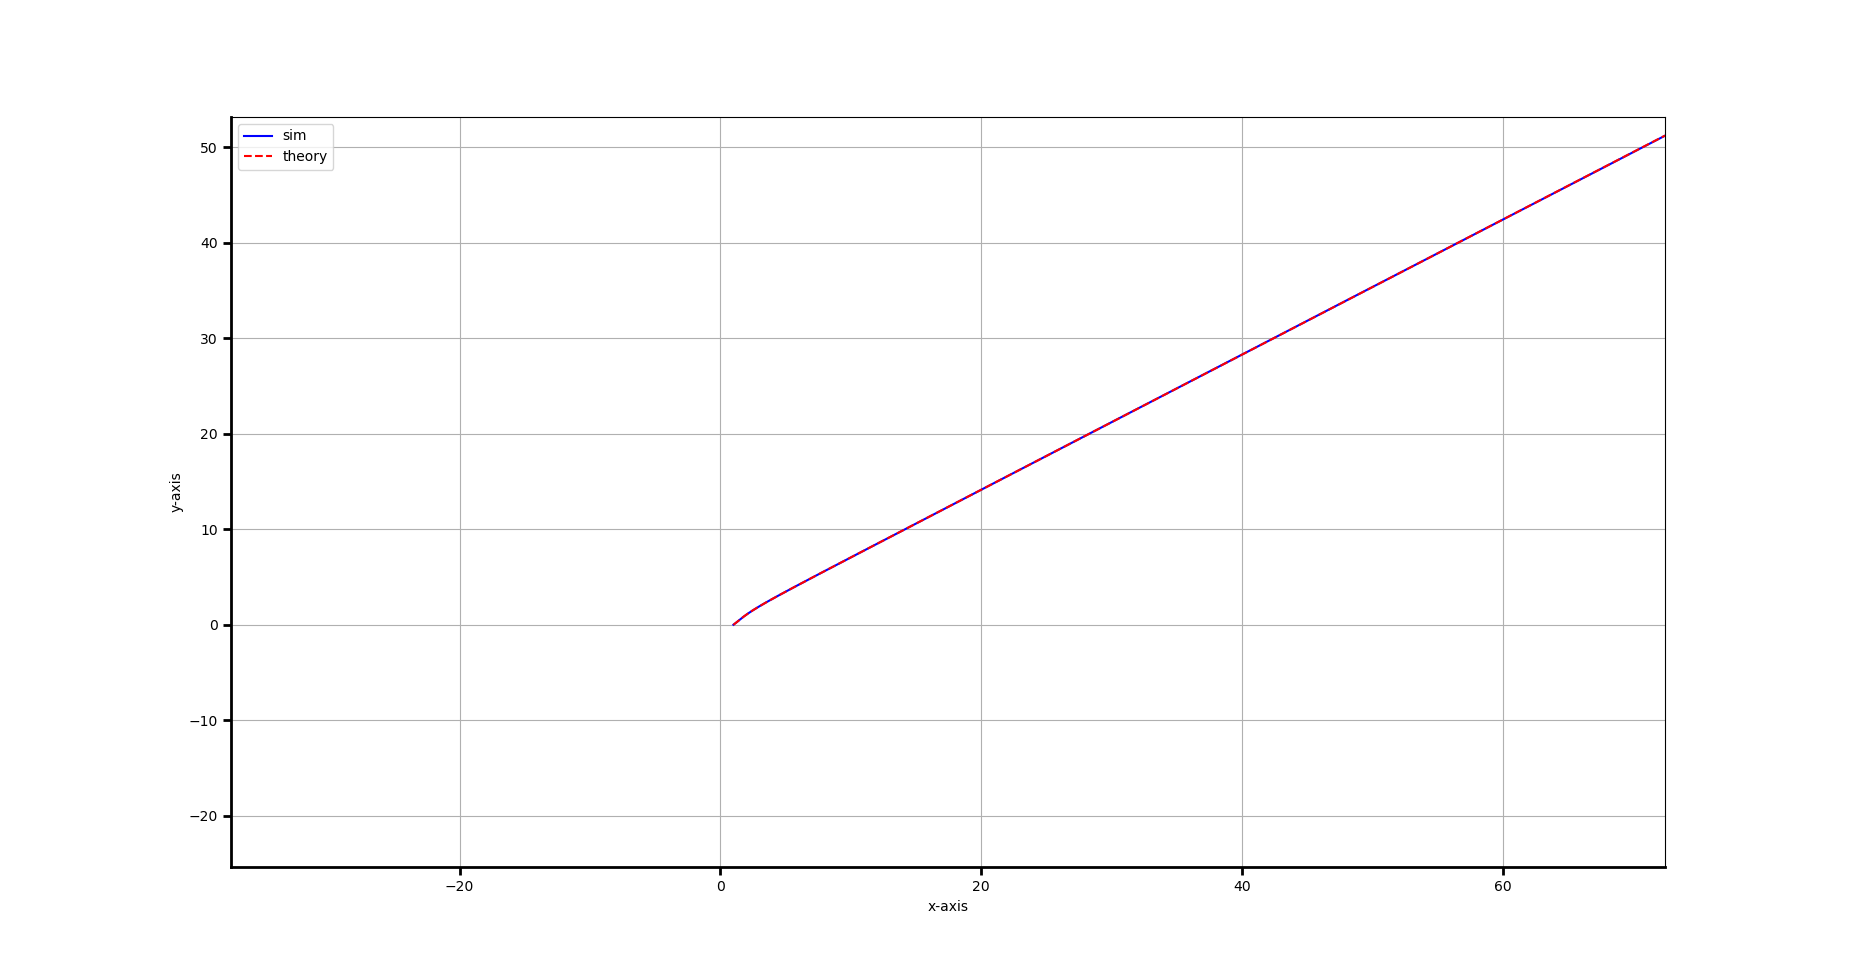
\includegraphics[width=\columnwidth]{figs/Figure_1.png}  
    \caption{Verification}
    \label{fig:example}  % Label for referencing
\end{figure}

\end{enumerate}

\end{document}
